% Figure from MATH 493 notes, section 50 (lecture 10/30, Jordan-Hoelder).
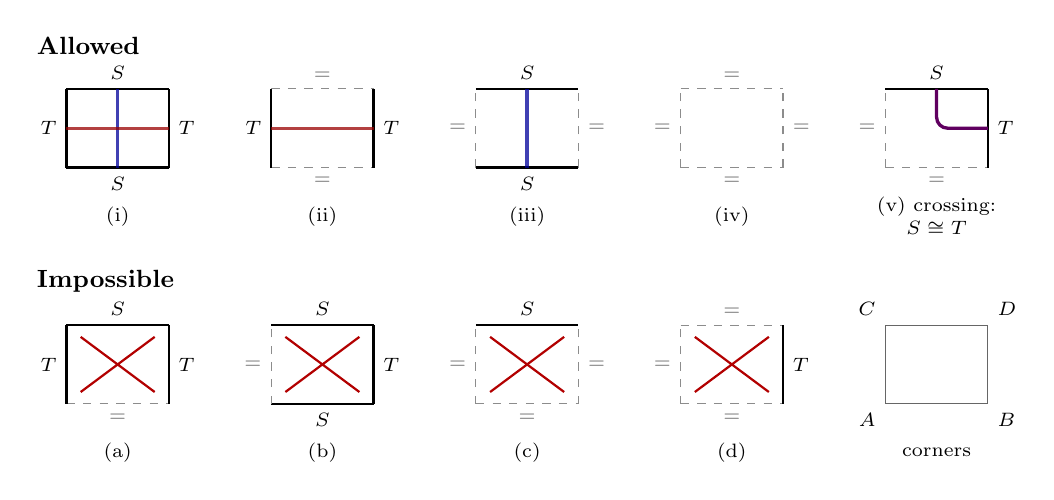
\begin{tikzpicture}[x=1cm, y=1cm]
\node[anchor=west, font=\small\bfseries] at (-0.5,1.55) {Allowed};
\draw[black, thick] (0.0, 1.0) -- (1.3, 1.0);
\node[above, black, font=\scriptsize] at (0.65,1.00) {$S$};
\draw[black, thick] (0.0, 0) -- (1.3, 0);
\node[below, black, font=\scriptsize] at (0.65,0.00) {$S$};
\draw[black, thick] (0.0, 0) -- (0.0, 1.0);
\node[left, black, font=\scriptsize] at (0.00,0.50) {$T$};
\draw[black, thick] (1.3, 0) -- (1.3, 1.0);
\node[right, black, font=\scriptsize] at (1.30,0.50) {$T$};
\draw[blue!60!black, very thick, opacity=0.75] (0.65,0.00) -- (0.65,1.00);
\draw[red!60!black, very thick, opacity=0.75] (0.00,0.50) -- (1.30,0.50);
\node[font=\scriptsize, align=center] at (0.65,-0.62) {(i)};
\draw[black!45, dashed] (2.6, 1.0) -- (3.9000000000000004, 1.0);
\node[above, black!55, font=\scriptsize] at (3.25,1.00) {$=$};
\draw[black!45, dashed] (2.6, 0) -- (3.9000000000000004, 0);
\node[below, black!55, font=\scriptsize] at (3.25,0.00) {$=$};
\draw[black, thick] (2.6, 0) -- (2.6, 1.0);
\node[left, black, font=\scriptsize] at (2.60,0.50) {$T$};
\draw[black, thick] (3.9000000000000004, 0) -- (3.9000000000000004, 1.0);
\node[right, black, font=\scriptsize] at (3.90,0.50) {$T$};
\draw[red!60!black, very thick, opacity=0.75] (2.60,0.50) -- (3.90,0.50);
\node[font=\scriptsize, align=center] at (3.25,-0.62) {(ii)};
\draw[black, thick] (5.2, 1.0) -- (6.5, 1.0);
\node[above, black, font=\scriptsize] at (5.85,1.00) {$S$};
\draw[black, thick] (5.2, 0) -- (6.5, 0);
\node[below, black, font=\scriptsize] at (5.85,0.00) {$S$};
\draw[black!45, dashed] (5.2, 0) -- (5.2, 1.0);
\node[left, black!55, font=\scriptsize] at (5.20,0.50) {$=$};
\draw[black!45, dashed] (6.5, 0) -- (6.5, 1.0);
\node[right, black!55, font=\scriptsize] at (6.50,0.50) {$=$};
\draw[blue!60!black, very thick, opacity=0.75] (5.85,0.00) -- (5.85,1.00);
\node[font=\scriptsize, align=center] at (5.85,-0.62) {(iii)};
\draw[black!45, dashed] (7.800000000000001, 1.0) -- (9.100000000000001, 1.0);
\node[above, black!55, font=\scriptsize] at (8.45,1.00) {$=$};
\draw[black!45, dashed] (7.800000000000001, 0) -- (9.100000000000001, 0);
\node[below, black!55, font=\scriptsize] at (8.45,0.00) {$=$};
\draw[black!45, dashed] (7.800000000000001, 0) -- (7.800000000000001, 1.0);
\node[left, black!55, font=\scriptsize] at (7.80,0.50) {$=$};
\draw[black!45, dashed] (9.100000000000001, 0) -- (9.100000000000001, 1.0);
\node[right, black!55, font=\scriptsize] at (9.10,0.50) {$=$};
\node[font=\scriptsize, align=center] at (8.45,-0.62) {(iv)};
\draw[black, thick] (10.4, 1.0) -- (11.700000000000001, 1.0);
\node[above, black, font=\scriptsize] at (11.05,1.00) {$S$};
\draw[black!45, dashed] (10.4, 0) -- (11.700000000000001, 0);
\node[below, black!55, font=\scriptsize] at (11.05,0.00) {$=$};
\draw[black!45, dashed] (10.4, 0) -- (10.4, 1.0);
\node[left, black!55, font=\scriptsize] at (10.40,0.50) {$=$};
\draw[black, thick] (11.700000000000001, 0) -- (11.700000000000001, 1.0);
\node[right, black, font=\scriptsize] at (11.70,0.50) {$T$};
\draw[violet!75!black, very thick, rounded corners=4pt] (11.05,1.00) -- (11.05,0.50) -- (11.70,0.50);
\node[font=\scriptsize, align=center] at (11.05,-0.62) {(v) crossing:\\ $S \cong T$};
\node[anchor=west, font=\small\bfseries] at (-0.5,-1.45) {Impossible};
\draw[black, thick] (0.0, -2.0) -- (1.3, -2.0);
\node[above, black, font=\scriptsize] at (0.65,-2.00) {$S$};
\draw[black!45, dashed] (0.0, -3.0) -- (1.3, -3.0);
\node[below, black!55, font=\scriptsize] at (0.65,-3.00) {$=$};
\draw[black, thick] (0.0, -3.0) -- (0.0, -2.0);
\node[left, black, font=\scriptsize] at (0.00,-2.50) {$T$};
\draw[black, thick] (1.3, -3.0) -- (1.3, -2.0);
\node[right, black, font=\scriptsize] at (1.30,-2.50) {$T$};
\draw[red!70!black, thick] (0.18,-2.85) -- (1.12,-2.15) (0.18,-2.15) -- (1.12,-2.85);
\node[font=\scriptsize, align=center] at (0.65,-3.62) {(a)};
\draw[black, thick] (2.6, -2.0) -- (3.9000000000000004, -2.0);
\node[above, black, font=\scriptsize] at (3.25,-2.00) {$S$};
\draw[black, thick] (2.6, -3.0) -- (3.9000000000000004, -3.0);
\node[below, black, font=\scriptsize] at (3.25,-3.00) {$S$};
\draw[black!45, dashed] (2.6, -3.0) -- (2.6, -2.0);
\node[left, black!55, font=\scriptsize] at (2.60,-2.50) {$=$};
\draw[black, thick] (3.9000000000000004, -3.0) -- (3.9000000000000004, -2.0);
\node[right, black, font=\scriptsize] at (3.90,-2.50) {$T$};
\draw[red!70!black, thick] (2.78,-2.85) -- (3.72,-2.15) (2.78,-2.15) -- (3.72,-2.85);
\node[font=\scriptsize, align=center] at (3.25,-3.62) {(b)};
\draw[black, thick] (5.2, -2.0) -- (6.5, -2.0);
\node[above, black, font=\scriptsize] at (5.85,-2.00) {$S$};
\draw[black!45, dashed] (5.2, -3.0) -- (6.5, -3.0);
\node[below, black!55, font=\scriptsize] at (5.85,-3.00) {$=$};
\draw[black!45, dashed] (5.2, -3.0) -- (5.2, -2.0);
\node[left, black!55, font=\scriptsize] at (5.20,-2.50) {$=$};
\draw[black!45, dashed] (6.5, -3.0) -- (6.5, -2.0);
\node[right, black!55, font=\scriptsize] at (6.50,-2.50) {$=$};
\draw[red!70!black, thick] (5.38,-2.85) -- (6.32,-2.15) (5.38,-2.15) -- (6.32,-2.85);
\node[font=\scriptsize, align=center] at (5.85,-3.62) {(c)};
\draw[black!45, dashed] (7.800000000000001, -2.0) -- (9.100000000000001, -2.0);
\node[above, black!55, font=\scriptsize] at (8.45,-2.00) {$=$};
\draw[black!45, dashed] (7.800000000000001, -3.0) -- (9.100000000000001, -3.0);
\node[below, black!55, font=\scriptsize] at (8.45,-3.00) {$=$};
\draw[black!45, dashed] (7.800000000000001, -3.0) -- (7.800000000000001, -2.0);
\node[left, black!55, font=\scriptsize] at (7.80,-2.50) {$=$};
\draw[black, thick] (9.100000000000001, -3.0) -- (9.100000000000001, -2.0);
\node[right, black, font=\scriptsize] at (9.10,-2.50) {$T$};
\draw[red!70!black, thick] (7.98,-2.85) -- (8.92,-2.15) (7.98,-2.15) -- (8.92,-2.85);
\node[font=\scriptsize, align=center] at (8.45,-3.62) {(d)};
\draw[black!60] (10.4,-3.0) rectangle (11.700000000000001,-2.0);
\node[below left, font=\scriptsize] at (10.4,-3.0) {$A$}; \node[below right, font=\scriptsize] at (11.700000000000001,-3.0) {$B$};
\node[above left, font=\scriptsize] at (10.4,-2.0) {$C$}; \node[above right, font=\scriptsize] at (11.700000000000001,-2.0) {$D$};
\node[font=\scriptsize, align=center] at (11.05,-3.62) {corners};
\end{tikzpicture}
